
\documentclass[compress]{beamer}

%\usepackage{beamerthemesplit}
\usepackage{xmpmulti}

\usepackage{booktabs}
\usepackage{graphicx,float,wrapfig, bbm}
\usepackage{amsfonts, bbold, comment}
\usepackage{mdwlist}
\usepackage{subfigure}
\usepackage{colortbl}

\usepackage{multirow}

\pgfdeclareimage[width=\paperwidth]{mybackground}{../../common/boulder.pdf}

\newcommand{\pos}[1]{{\texttt{#1}}}
\newcommand{\e}[2]{\mathbb{E}_{#1}\left[ #2 \right] }
\newcommand{\ind}[1]{\mathbb{I}\left[ #1 \right] }
\newcommand{\abr}[1]{\textsc{#1} }
\newcommand{\ex}[1]{\mbox{exp}\left\{ #1\right\} }
\newcommand{\g}{\, | \,}
\newcommand{\citename}[1]{#1 }

\newcommand{\gfxs}[2]{
\begin{center}
	\includegraphics[width=#2\linewidth]{simtrans/#1}
\end{center}
}

\newcommand{\gfxq}[2]{
\begin{center}
	\includegraphics[width=#2\linewidth]{qb/#1}
\end{center}
}


\usetheme[bullet=circle,                     % Use circles instead of squares for bullets.
          titleline=true,                    % Show a line below the frame title.
          showdate=true,                     % show the date on the title page
          alternativetitlepage=true,         % Use the fancy title page.
          titlepagelogo=general_figures/culogo,              % Logo for the first page.
          % Logo for the header on first page.
          headerlogo=general_figures/boulder_cs,
          ]{UCBoulder}

\usecolortheme{ucdblack}
\title[Thinking on Your Feet]{Thinking on your Feet: Reinforcement Learning for Incremental
Language Tasks}
\author{ Jordan Boyd-Graber}
\date{Fall 2015}

\institute[Boulder] % (optional, but mostly needed)
{University of Colorado Boulder}

\AtBeginSection[] % "Beamer, do the following at the start of every section"
{ \begin{frame} \frametitle{Outline} % make a frame titled "Outline"
\tableofcontents[currentsection] % show TOC and highlight current section
\end{frame} }

\begin{document}

\frame{
\titlepage
\tiny
}


\begin{frame}{Nuremburg Trials}

\begin{columns}

\column{.5\linewidth}

    \gfxs{nuremberg_trials}{1.0}

\column{.5\linewidth}

    \begin{itemize}
        \item Dozens of defendants
        \item Judges from four nations (three languages)
\pause
        \item Status quo: speak, then translate
\pause
        \item After Nuremberg, simultaneous translations became the
          norm
\pause
        \item Long wait $\rightarrow$ bad conversation
     \end{itemize}

\end{columns}

\end{frame}



\begin{frame}{Algorithms that think on their feet}

\begin{columns}

  \column{.65\linewidth}
  \begin{itemize}
     \item Algorithms that process examples \emph{one word at a time}
       \begin{itemize}
         \item Simultaneous machine translation
         \item Trivia games
       \end{itemize}
      \item Similar structure
        \begin{itemize}
          \item Prediction
          \item Policy
        \end{itemize}
  \end{itemize}

  \column{.3\linewidth}

  \gfxs{nuremberg_translators}{.7}
  \gfxq{quizbowl}{.7}

\end{columns}

\end{frame}



\begin{frame}{Very Different Tasks, Common Foundation}

\begin{columns}
\column{.5\linewidth}
  \gfxs{pancake_robot}{.4}
  \begin{center}
  \end{center}
  
  \column{.5\linewidth}
  \begin{itemize}
    \item Reinforcement learning
    \item Machine learning / robotics framework
    \item Underused in NLP
  \end{itemize}
\end{columns}

\vspace{-.5cm}

  \begin{center}
\begin{tabular}{ccc}
\hline
  & QA & MT \\
\hline
{\bf State} & Words Seen & Foreign Words Seen \\
{\bf Reward} & Answer Accuracy & Translation Quality \\
{\bf Actions} & Answer / Wait & Translate / Wait \\
\hline
\end{tabular}

  \end{center}

\end{frame}

\section{Quiz Bowl}

\begin{frame}
	\frametitle{Humans doing Incremental Classification}
	\begin{columns}

	\column{.5\linewidth}
	\begin{itemize}
		\item Game called ``quiz bowl''
		\item Two teams play each other
		\begin{itemize}
			\item Moderator reads a question
			\item When a team knows the answer, they signal (``buzz'' in)
			\item If right, they get points; otherwise, rest of the question is read to the other team
		\end{itemize}
		\item Hundreds of teams in the US alone
                \only<2>{\item Example \dots}
	\end{itemize}

	\column{.5\linewidth}
	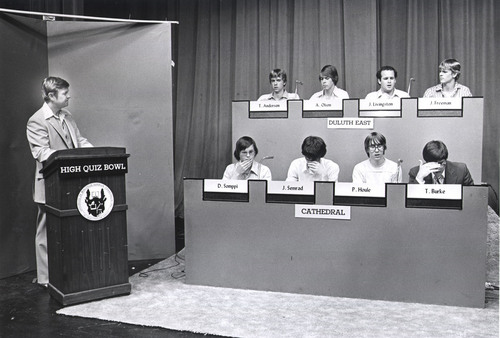
\includegraphics{qb/quizbowl}

	\end{columns}

\end{frame}

\begin{frame}[t]
\frametitle{Sample Question}
	\frametitle{Sample Question}

With Leo Szilard, he invented a doubly-eponymous \only<2->{refrigerator with no moving parts. He did not take interaction with neighbors into account when formulating his theory of} \only<3->{heat capacity, so} \only<4->{Debye adjusted the theory for low temperatures. His} \only<4->{summation convention automatically sums repeated indices in tensor products. His name is attached to the A and B coefficients} \only<5->{for spontaneous and stimulated emission, the subject of one of his multiple groundbreaking 1905 papers. He further developed the model of statistics sent to him by} \only<6->{Bose to describe particles with integer spin. For 10 points, who is this German physicist best known for formulating the} \only<7->{special and general theories of relativity?} \\
\vspace{1cm}
\only<8->{ {\bf Albert \underline{Einstein}}}

\only<9->{
\vspace{-6cm}

\begin{block}{Faster = Smarter}

  \begin{enumerate}
    \item Colorado School of Mines
    \item Cornell University
    \item Brigham Young University
    \item California Institute of Technology
    \item Peking University
    \item Harvey Mudd College
    \item Darmstadt University
    \item University of Colorado
  \end{enumerate}


\end{block}
}


\end{frame}



\begin{frame}
	\frametitle{Humans doing Incremental Classification}

	\begin{columns}
		\column{.5\linewidth}

		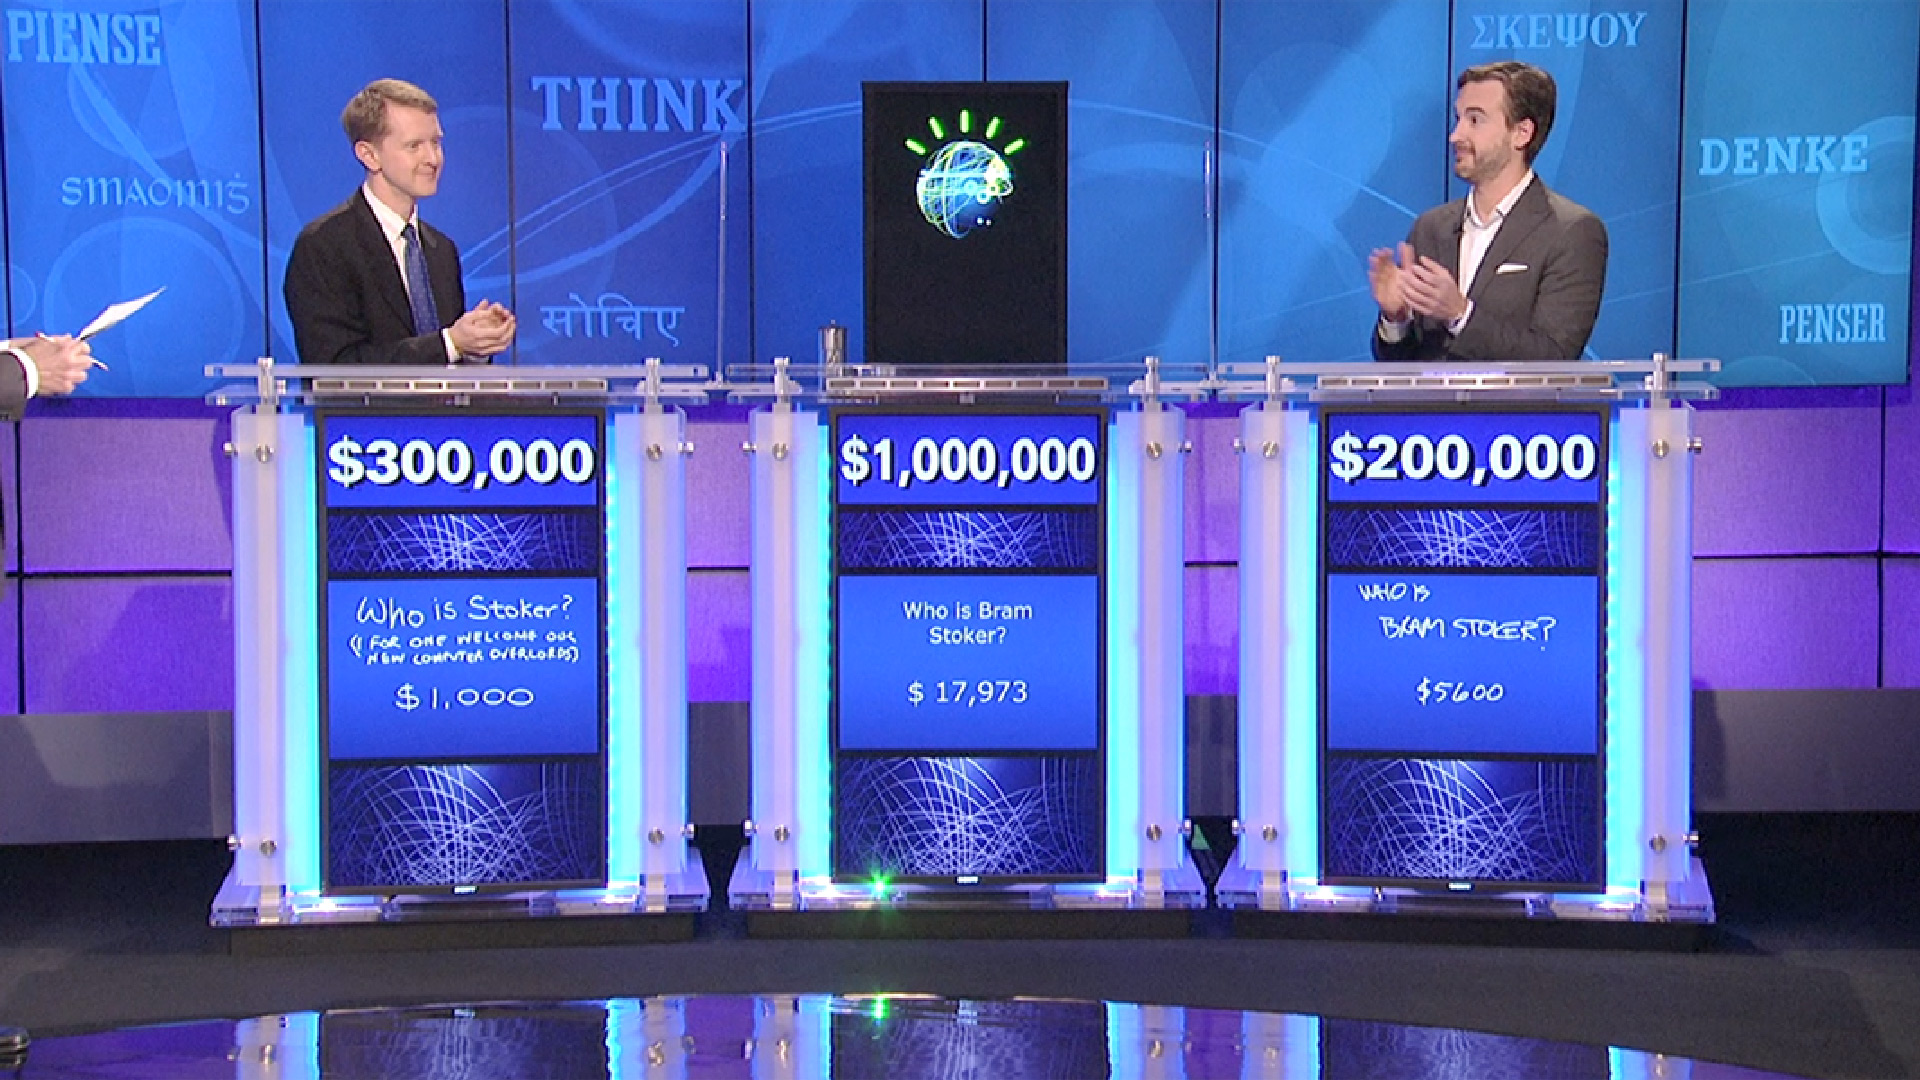
\includegraphics[width=1.0\linewidth]{qb/jeopardy}


		\column{.5\linewidth}
		\begin{itemize}
			\item This is {\bf not} Jeopardy \cite{ferruci-10}
			\item There are buzzers, but players only buzz
                          at the question end
			\item Doesn't discriminate knowledge
			\item Quiz bowl is pyramidal
                        \item Watson must decide to answer {\bf once}, after
                          complete question
                        \item Quiz Bowl: decide after each word
		\end{itemize}

	\end{columns}

\end{frame}



\begin{frame}
	\frametitle{Humans doing Incremental Classification}

	\begin{itemize}
		\item Thousands of questions are written every year
		\item Large question databases
		\item Teams practice on these questions (some online, e.g. IRC)
		\item How can we learn from this?
	\end{itemize}

\end{frame}

\begin{frame}{}

  \begin{columns}
    \column{.5\linewidth}
        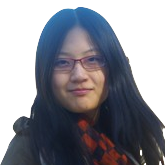
\includegraphics[width=0.7\linewidth]{general_figures/hehe} \\
        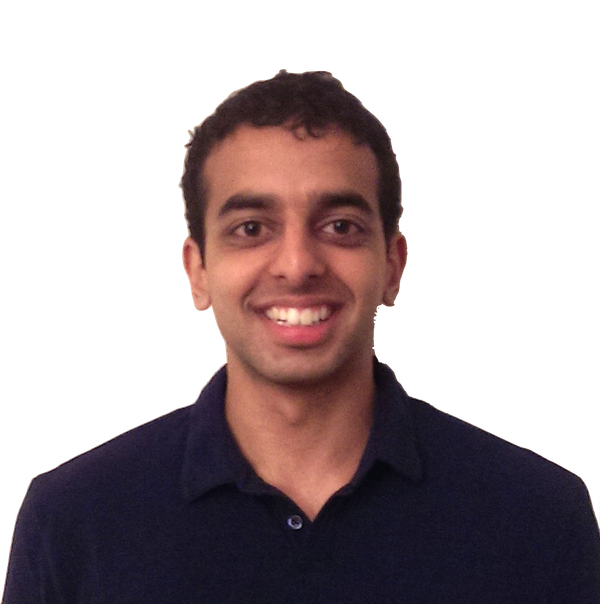
\includegraphics[width=0.7\linewidth]{general_figures/mohit}
    \column{.5\linewidth}
        \begin{block}{{\bf
              \href{http://cs.colorado.edu/~jbg//docs/qb_emnlp_2012.pdf}{Besting
                the Quiz Master: Crowdsourcing Incremental
                Classification Games}}} 

          {\bf Jordan Boyd-Graber}, He He, and Hal {Daum\'{e} III}. \emph{Empirical Methods in Natural Language Processing}, 2012
        \end{block}

        \begin{block}{ {\bf \href{http://cs.colorado.edu/~jbg//docs/2014_emnlp_qb_rnn.pdf}{A Neural Network for Factoid Question Answering over Paragraphs}}}
\underline{\href{http://cs.umd.edu/~miyyer/}{Mohit Iyyer}}, {\bf Jordan Boyd-Graber}, Leonardo Claudino, Richard Socher, and Hal {Daum\'{e} III}.  \emph{Empirical Methods in Natural Language Processing}, 2014
        \end{block}


  \end{columns}
\end{frame}


\begin{frame}
	\frametitle{System for Incremental Classifiers}

	\begin{itemize}
		\item Treat this as a MDP
		\item Action: {\bf buzz} now or {\bf wait}
                     \pause
                    \begin{enumerate}
                  \item {\bf Content Model} is constantly generating guesses
                     \item {\bf Oracle} provides examples where it is correct
                   \item The {\bf Policy} generalizes to test data
                       \item {\bf Features} represent our state
                    \end{enumerate}
	\end{itemize}
\begin{block}{}
  \begin{center}
    \vspace{-.5cm}
    \begin{tabular}{cccc}
      \alert<3->{content model} & oracle & policy & features \\
    \end{tabular}
    \vspace{-.5cm}
  \end{center}
\end{block}
\end{frame}


\begin{frame}{Content Model}

\begin{block}{}
  \begin{center}
    \vspace{-.5cm}
    \begin{tabular}{cccc}
      \alert{content model} & oracle & policy & features \\
    \end{tabular}
    \vspace{-.5cm}
  \end{center}
\end{block}


  \begin{itemize}
   \item Bayesian generative model with answers as latent state
         \item Unambiguous Wikipedia pages
           \item Unigram term weightings (na\"ive Bayes, BM25)
    \item Maintains posterior distribution over guesses
    \item Always has a guess of what it should answer
      \begin{itemize}
        \item policy will tell us when to trust it
       \end{itemize}

  \end{itemize}
\end{frame}

\begin{frame}{Vector Space Model}

  \only<1>{\gfxq{unigram_models_0}{.8}}
  \only<2>{\gfxq{unigram_models_1}{.8}}
  \only<3>{\gfxq{unigram_models_2}{.8}}
  \only<4>{\gfxq{unigram_models_3}{.8}}
  \only<5>{\gfxq{unigram_models_4}{.8}}
  \only<6>{\gfxq{unigram_models_5}{.8}}
  \only<7>{\gfxq{unigram_models_6}{.8}}
  \only<8>{\gfxq{unigram_models_7}{.8}}
  \only<9>{\gfxq{unigram_models_8}{.8}}


\end{frame}


\begin{frame}{How can we do better?}

  \begin{itemize}
    \item Use order of words in a sentence ``this man shot Lee Harvey Oswald'' very different from ``Lee Harvey Oswald shot this man''
    \item Use relationship between questions (``China'' and
      ``Taiwan'')
    \item Use learned features and dimensions, not the words we start with
      \pause
    \item Recursive Neural Networks~\cite{socher-12}
    \item First-time a \emph{learned} representation has been applied
      to question answering
  \end{itemize}

\end{frame}

\begin{frame}{Using Compositionality}

  \only<1-2>{\gfxq{rnn_11}{.8}}
  \only<3>{\gfxq{rnn_10}{.8}}
  \only<4>{\gfxq{rnn_9}{.8}}
  \only<5>{\gfxq{rnn_8}{.8}}
  \only<6>{\gfxq{rnn_7}{.8}}
  \only<7>{\gfxq{rnn_6}{.8}}

  \only<8>{\gfxq{rnn_recursive_1}{.8}}
  \only<9>{\gfxq{rnn_recursive_2}{.8}}
  \only<10>{\gfxq{rnn_recursive_3}{.8}}

  \only<11>{\gfxq{rnn_5}{.8}}
  \only<12>{\gfxq{rnn_4}{.8}}
  \only<13>{\gfxq{rnn_3}{.8}}
  \only<14>{\gfxq{rnn_2}{.8}}

\end{frame}


\begin{frame}{Training}

  \begin{columns}
    \column{.5\linewidth}
      \begin{itemize}
        \item Initialize embeddings from \textsc{word2vec}
        \item Randomly initialize composition matrices
        \item Update using \textsc{warp}
          \begin{itemize}
            \item Randomly choose an instance
            \only<2->{\item Look where it lands}
            \only<4->{\item Has a correct answer}
            \only<5->{\item Wrong answers may be closer}
            \only<6->{\item Push away wrong answers
            \item Bring correct answers closer}
          \end{itemize}
      \end{itemize}

    \column{.5\linewidth}

      \only<1>{\gfxq{warp_training_5}{.8}}
      \only<2>{\gfxq{warp_training_4}{.8}}
      \only<3>{\gfxq{warp_training_3}{.8}}
      \only<4>{\gfxq{warp_training_2}{.8}}
      \only<5>{\gfxq{warp_training_1}{.8}}
      \only<6>{\gfxq{warp_training_0}{.8}}
  \end{columns}

\end{frame}


\begin{frame}{Oracle}
\begin{block}{}
  \begin{center}
    \vspace{-.5cm}
    \begin{tabular}{cccc}
      content model & \alert{oracle} & policy & features \\
    \end{tabular}
    \vspace{-.5cm}
  \end{center}
\end{block}
\begin{center}
  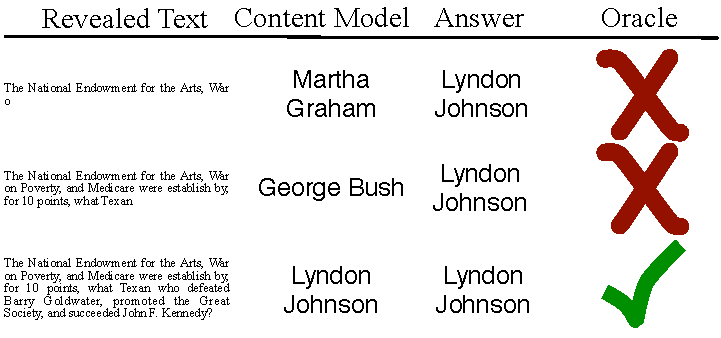
\includegraphics[width=0.8\linewidth]{qb/oracle}
\end{center}

\begin{itemize}
  \item As each token is revealed, look at content model's guess
    \item If it's right, positive instance; otherwise negative
      \item Nearly optimal policy to buzz whenever correct (upper bound)
\end{itemize}

\end{frame}

\begin{frame}{Policy}

\begin{block}{}
  \begin{center}
    \vspace{-.5cm}
    \begin{tabular}{cccc}
      content model & oracle & \alert{policy} & features \\
    \end{tabular}
    \vspace{-.5cm}
  \end{center}
\end{block}

 \begin{itemize}
    \item Mapping: state $\mapsto$ action
    \item Use oracle as example actions
    \item Learned as classifier \cite{langford-05}
    \item At test time, use the same features as for training
      \begin{itemize}
        \item Question text (so far)
        \item Guess
        \item Posterior distribution
        \item Change in posterior
      \end{itemize}
\end{itemize}

\end{frame}



\begin{frame}[t]{Features (by example)}

\only<1-3>{
\begin{block}{}
  \begin{center}
    \vspace{-.5cm}
    \begin{tabular}{cccc}
      content model & oracle & policy & \alert{features} \\
    \end{tabular}
    \vspace{-.5cm}
  \end{center}
\end{block}
\vspace{.5cm}
}

\only<4->{\vspace{-1.5cm}}

  \begin{columns}[T]
    \column{.3\linewidth}

    \only<1->{ 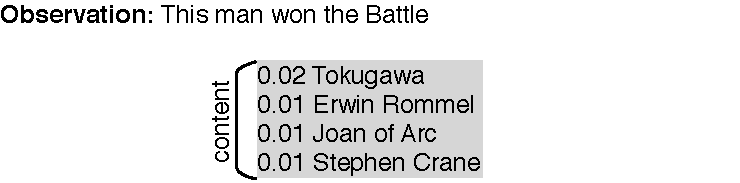
\includegraphics[width=2\linewidth]{qb/feature_ex_l_1} \\ }
    \vspace{.5cm}
    \only<4->{ 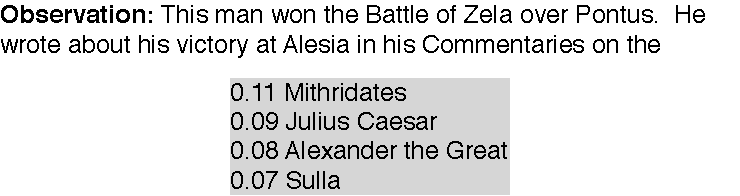
\includegraphics[width=2\linewidth]{qb/feature_ex_l_2}  \\ }
    \vspace{.5cm}
    \only<7->{ 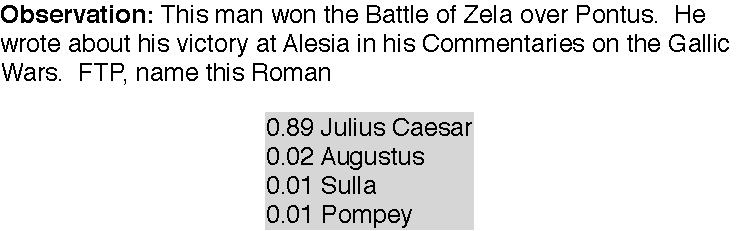
\includegraphics[width=2\linewidth]{qb/feature_ex_l_3}  \\ }


    \column{.68\linewidth}
    \vspace{-.5cm}
    \only<2->{ 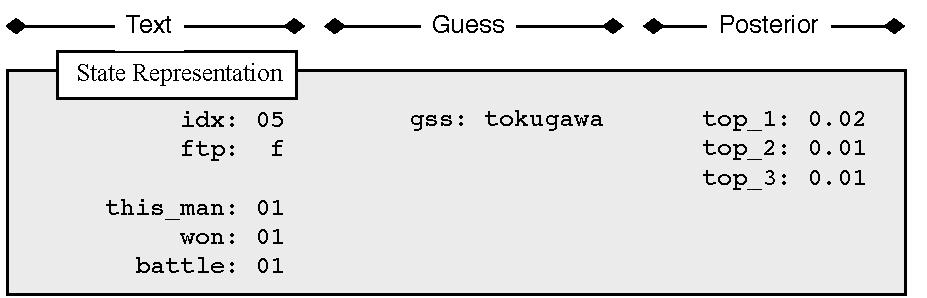
\includegraphics[width=.85\linewidth]{qb/feature_ex_r_1} \\ }
    \only<3->{ \vspace{-.5cm} \hspace{.5cm} 
\includegraphics[width=.1\linewidth]{qb/feature_ex_wait}  \\ }
    \only<5->{ 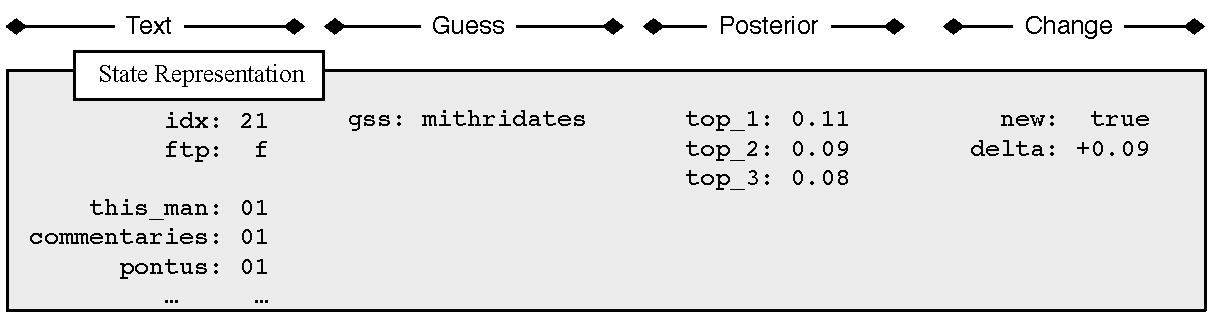
\includegraphics[width=\linewidth]{qb/feature_ex_r_2} \\ }
    \only<6->{ \vspace{-.5cm} \hspace{.5cm}
\includegraphics[width=.1\linewidth]{qb/feature_ex_wait}  \\ }
    \only<8->{ 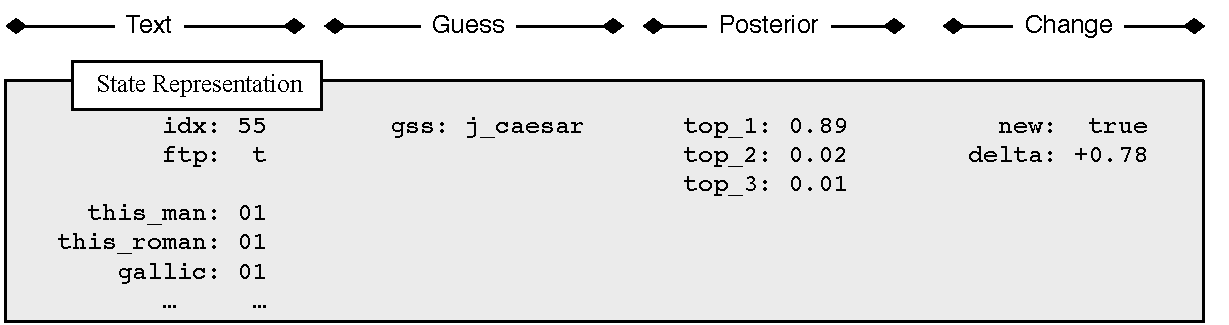
\includegraphics[width=\linewidth]{qb/feature_ex_r_3} \\ }
    \only<9->{ \vspace{-.5cm} \hspace{.5cm} 
\includegraphics[width=.1\linewidth]{qb/feature_ex_buzz}  \\ }
    \only<9->{Answer: {\bf Julius Caesar}}
  \end{columns}

\end{frame}



\begin{frame}{Simulating a Game}
		\begin{itemize}
			\item Present tokens incrementally to algorithm, see where it buzzes
			\item Compare to where humans buzzed in
			\item Payoff matrix (wrt Computer)
			\begin{center}
\begin{tabular}{lccr}
& Computer & Human & Payoff \\
\hline
1 & first and wrong & right & $-15$ \\
2 & --- & first and correct & $-10$ \\
3  & first and wrong & wrong & $-5$ \\
4 & first and correct & --- & $+10$ \\
5 & wrong & first and wrong & $+5$ \\
6 & right & first and wrong & $+15$ \\
\hline
\end{tabular}
			\end{center}
		\end{itemize}
\end{frame}

\begin{frame}
\frametitle{Interface}

\begin{columns}

	\column{0.5\linewidth}

	\begin{center}
		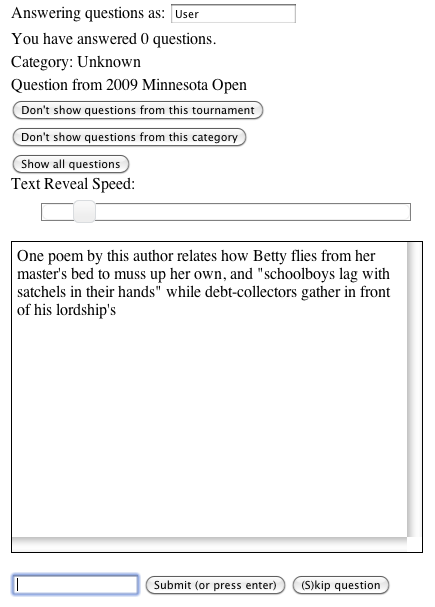
\includegraphics[width=0.8\linewidth]{qb/screenshot}
	\end{center}

	\column{0.5\linewidth}
	\only<1>{
	\begin{itemize}
		\item Users could ``veto'' categories or tournaments
		\item Questions presented in canonical order
		\item Approximate string matching (w/ override)
	\end{itemize}
	}

	\only<2>{
	\begin{itemize}
		\item Started on Amazon Mechanical Turk
		\item 7000 questions were answered in the first day
		\item Over 43000 questions were answered in the space of two weeks
		\item Total of 461 unique users
		\item Leaderboard to encourage users
	\end{itemize}
	}

\end{columns}
\end{frame}


\begin{frame}{Embedding}

  \gfxq{embedding}{1.0}

\end{frame}

\begin{frame}{Comparing \textsc{rnn} to \textsc{bow}}

\begin{center}
\begin{tabular}{lrrrrrr}
\hline
& \multicolumn{3}{c}{History} & \multicolumn{3}{c}{Literature}\\
Model    & Sent 1 & Sent 2 & Full & Sent 1 & Sent 2 & Full \\
\hline
\textsc{bow-qb} & 37.5 & 65.9 & 71.4 & 27.4 & 54.0 & 61.9 \\
\alert<2>{\textsc{rnn}} & \bf 47.1 & \bf 72.1 & \bf 73.7 & \bf 36.4 & \bf 68.2 & \bf 69.1 \\
\hline
\alert<3>{\textsc{bow-wiki}} & 53.7 & 76.6 & 77.5 & 41.8 & 74.0 & 73.3 \\
\alert<4>{\textsc{combined}} & \bf 59.8 & \bf 81.8 & \bf 82.3 & \bf 44.7 & \bf 78.7 & \bf 76.6 \\
\hline
\end{tabular}
\end{center}

Percentage accuracy of different vector-space models.

\end{frame}

\begin{frame}{Now we're able to beat humans}

  \gfxq{human_history}{1.0}

\end{frame}

\begin{frame}{Examining vectors}

  \only<1>{\gfxq{mann}{.65}}
  \only<2>{\gfxq{cabot}{.6}}

\end{frame}

\begin{frame}{Experiment 1}

		\begin{columns}
			\column{.25\linewidth}
				\gfxq{colby_jeo}{1.0} 
                                Colby Burnett:
                                \$375,000
			\column{.25\linewidth}
				\gfxq{ben_jeo}{1.0}
                                Ben Ingram:
                                \$427,534
			\column{.25\linewidth}
				\gfxq{alex_jeo}{1.0}
                                Alex Jacobs: \$151,802
			\column{.25\linewidth}
				\gfxq{kristin_jeo}{1.0}
                                Kristin Sausville: \$95,201
		\end{columns}

                \pause

                
                \begin{center}
                End result: 200-200 tie!
                \end{center}

\end{frame}

\begin{frame}{Experiment 2}

\gfxq{jennings}{.7}

\begin{itemize}
  \item More data helps
  \item Improving country pages specifically
  \item Still weak on popular culture
  \item Limited set of answers
\end{itemize}

\end{frame}


\begin{frame}{Building on this Foundation}

  \begin{itemize}
    \item Using Wikipedia: Deep Averaging Networks~\cite{iyyer-15}
    \item New network structures: capturing coreference~\cite{guha-15}
    \item Incorporating additional information: story plots
  \end{itemize}

\end{frame}

\section{Simultaneous Translation}

\begin{frame}{Simultaneous translation is the norm}

  \begin{columns}
    \column{.5\linewidth}
       \gfxs{nuremberg_translators}{.9}
    \column{.5\linewidth}
       \begin{itemize}
         \item Rigorous training
         \item Technological sophistication
         \item Long way from ``sentence at a time''
       \end{itemize}
  \end{columns}

\end{frame}

\begin{frame}{Why simultaneous translation really hard is}

  \begin{columns}
    \column{.5\linewidth}
      \begin{itemize}
        \item Many languages are \textsc{sov}
        \item \alert<2>{German}, Japanese, Farsi, Korean,
          \alert<3>{Yiddish}
        \item<4-> First learned system for simulatenous translation
      \end{itemize}
    \column{.5\linewidth}
      \gfxs{yoda}{.6}
  \end{columns}

  \centering

\only<4-5>{
\vspace{1cm}

\begin{tabular}{c@{ }c@{ }c@{ }c@{ }c@{ }c@{ }c@{ }l}
ich & bin & mit & dem & Zug & nach & Ulm & {\bf gefahren} \\
I & am & with & the & train & to & Ulm & {\bf traveled} \\
\hline
I & \multicolumn{6}{c}{\emph{(\dots\dots waiting\dots\dots)}} & {\bf traveled} by train to Ulm \\
\end{tabular}
}

\only<6>{
  \gfxs{en_ja_example}{.8}
}

\end{frame}


\begin{frame}{}

  \begin{columns}
    \column{.5\linewidth}
        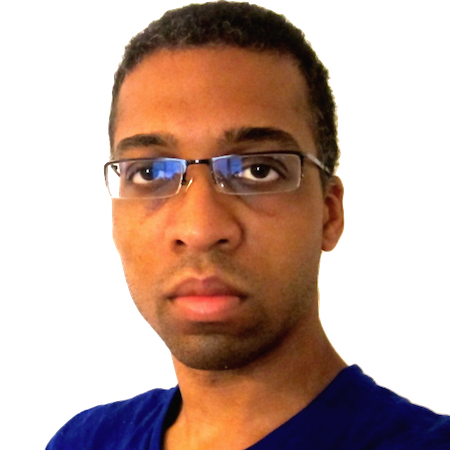
\includegraphics[width=0.9\linewidth]{general_figures/alvin}
    \column{.5\linewidth}
        \begin{block}{ {\bf \href{http://cs.colorado.edu/~jbg//docs/2014_emnlp_simtrans.pdf}{Don't Until the Final Verb Wait: Reinforcement Learning for Simultaneous Machine Translation}}}
\underline{\href{http://www.umiacs.umd.edu/~alvin/}{Alvin Grissom II}}, {\bf Jordan Boyd-Graber}, He He, John Morgan, and Hal {Daum\'{e} III}.  \emph{Empirical Methods in Natural Language Processing}, 2014
        \end{block}
  \end{columns}
\end{frame}

\begin{frame}{Solution: Predicting the Verb}

\begin{columns}

\column{.5\linewidth}
  \begin{itemize}
    \item If we can figure out the verb, we can ``complete'' the
      sentence
    \item This is provided by language models that can predict the
      next word in a sentence
    \item Instead, we'll predict the verb
  \end{itemize}

\column{.5\linewidth}

\gfxs{autocomplete}{.8}

\end{columns}

\end{frame}


\begin{frame}{Language Models of Verbs}

  \only<1>{\gfxs{verb_corpus_1}{.9}}
  \only<2>{\gfxs{verb_corpus_2}{.9}}
  \only<3>{\gfxs{verb_corpus_3}{.9}}

\end{frame}

\begin{frame}{Predicting the Verb}
\begin{itemize}
  \item Build language model for every verb
  \item Then, for any input text $x$ we can make a prediction of the verb
\begin{equation}
  \arg\max_v p(v) \prod_{i=1}^t p(x_i \g v, x_{i-n+1:i-1})
\end{equation}
\pause
  \item Most of these predictions will be totally wrong (18\%
    accuracy) \dots
  \item leading to horrible translations
\end{itemize}
\end{frame}

\begin{frame}{States and Actions}

  \begin{itemize}
    \item State
      \begin{itemize}
        \item The words we've seen
        \item Predictions
      \end{itemize}
      \pause
    \item Actions (more complicated than Quiz Bowl)
      \begin{itemize}
        \item Wait
        \item \alert<3>{Predict Verb and Translate}
        \item \alert<3>{Commit to Translation}
      \end{itemize}
    \end{itemize}
\end{frame}

\begin{frame}{Translations}
  \begin{itemize}
    \item Assume a ``black box''
    \item German in, English out
  \end{itemize}

\end{frame}

\begin{frame}{Consensus Translation}

  \only<1>{\begin{center}
``German in, English out'' black box
      \end{center}}

  \only<2>{\gfxs{consensus_0}{.8}}
  \only<3>{\gfxs{consensus_1}{.8}}
  \only<4>{\gfxs{consensus_2}{.8}}
  \only<5>{\gfxs{consensus_3}{.8}}
  \only<6>{\gfxs{consensus_4}{.8}}

\end{frame}

\begin{frame}{Scoring one Translation}
  \begin{center}
    Bilingual Evaluation Understudy (BLEU)
\end{center}
  \only<1>{\gfxs{bleu_ex}{.8}}
  \only<2>{\gfxs{bleu_correlation}{.6}}
\end{frame}


\begin{frame}{Scoring a series of Translations}
  \begin{center}
    Bilingual Evaluation Understudy (BLEU)
\end{center}
  \only<1>{\gfxs{integral_0}{.95}}
  \only<2>{\gfxs{integral_1}{.95}}
\end{frame}



\begin{frame}{Comparing Policies}

  \only<1-7>{\vspace{4.75cm}}
  \only<8-14>{\vspace{3.3cm}}
  \only<15-21>{\vspace{2cm}}

  \only<1,8,15,22>{\gfxs{reward_example_0}{.8}}
  \only<2,9,16,23>{\gfxs{reward_example_1}{.8}}
  \only<3,10,17,24>{\gfxs{reward_example_2}{.8}}
  \only<4,11,18,25>{\gfxs{reward_example_3}{.8}}
  \only<5,12,19,26>{\gfxs{reward_example_4}{.8}}
  \only<6,13,20,27>{\gfxs{reward_example_5}{.8}}
  \only<7,14,21,28>{\gfxs{reward_example_6}{.8}}
\end{frame}




\begin{frame}{Imitation Learning}

  \begin{columns}
    \column{.5\linewidth}
       \gfxs{imitation_fold}{.8}
       \gfxs{imitation_drive}{.8}
    \column{.5\linewidth}
    \begin{itemize}
      \item Given all the predictions that we make (and the resulting
        translations) \dots
      \item Discover the optimal in hindsight policies
      \item Goal: Teach our algorithm to think on its feet
      \item Challenge: Represent states in a way that will generalize
    \end{itemize}

  \end{columns}

\end{frame}


\begin{frame}{How do we find a good policy?}

  \only<1>{\gfxs{searn_7}{.8}}
  \only<2>{\gfxs{searn_6}{.8}}
  \only<3>{\gfxs{searn_5}{.8}}
  \only<4>{\gfxs{searn_4}{.8}}
  \only<5>{\gfxs{searn_3}{.8}}
  \only<6>{\gfxs{searn_2}{.8}}
  \only<7>{\gfxs{searn_1}{.8}}
\end{frame}


\begin{frame}{How do we find a good policy?}

  \begin{itemize}
    \item Find optimal policies through dynamic programming $\pi_0
      \equiv \pi*$
    \item Represent states $s$ through a feature vector $\vec f(s)$
      \pause
    \item Until convergence:
      \begin{itemize}
        \item Generate examples of state action pairs: $(\pi_t(s), s)$
        \item Create a classifier that maps states to actions (an
          apprentice policy) $h_t: f(s) \mapsto A$ \only<3->{(Loss of
            classifier is the negative reward)}
    \item Interpolate learned classifier $\pi_{t+1} = \lambda \pi_t +
      (1-\lambda) h_t$
  \end{itemize}
  \end{itemize}

\only<4->{
  \begin{center}
    \textsc{searn}: \underline{Se}arching to L\underline{earn}
    (Daum\'e \& Marcu, 2006)
    \end{center}
}
\end{frame}


\begin{frame}{Experimental Setup}

  \begin{itemize}
    \item \textsc{denews} corpus
      \begin{itemize}
        \item News snippets
        \item Some formulaic
        \item Some surprising
      \end{itemize}
    \item Only verb-final sentences
    \item Some compromises with translation system (to make sure verbs appeared)
  \end{itemize}

\end{frame}



\begin{frame}{Comparing Policies}

  \gfxs{cummulative}{.6}

\end{frame}

\begin{frame}{Learned Policy with Accumulated Reward}

  \only<1>{\gfxs{compare_line_batch}{.8}}
  \only<2>{\gfxs{compare_line_batch_monotone}{.8}}
  \only<3>{\gfxs{compare_line_batch_monotone_opt}{.8}}
  \only<4>{\gfxs{compare_line_all}{.8}}
\end{frame}


\begin{frame}{Example Sentence}

  \gfxs{ex_imperfect}{.7}

  \pause

  But we're still at the mercy of our translation black box

\end{frame}


\begin{frame}{}

  \begin{columns}
    \column{.5\linewidth}
        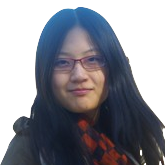
\includegraphics[width=0.8\linewidth]{general_figures/hehe}
    \column{.5\linewidth}
        \begin{block}{ {\bf \href{http://cs.colorado.edu/~jbg//docs/2015_emnlp_rewrite.pdf}{Syntax-based Rewriting for Simultaneous Machine Translation}}}
He He, Alvin Grissom II, {\bf Jordan Boyd-Graber}, and Hal {Daum\'{e} III}.  \emph{Empirical Methods in Natural Language Processing}, 2015
        \end{block}
  \end{columns}
\end{frame}

\begin{frame}{How can we make MT better?}

  \gfxs{en_ja_example}{.9}

  \pause

  \begin{itemize}
    \item In a perfect world, we'd use interpretation data
      \pause
      \item Very rare, and low quality in other ways
      \pause
    \item But can we \emph{rewrite} batch translations?
  \end{itemize}

\end{frame}

\begin{frame}{Are there enough opportunities?}


\begin{center}
\begin{tabular}{lcccc}
\toprule
& \alert<2>{verb} & \alert<3>{voice} & \alert<4>{noun} & \alert<5>{clauses} \\
\midrule
Applicable \% & \only<2->{39.9} & \only<3->{50.0} & \only<4->{26.4} & \only<5->{4.8} \\
Accepted \% & \only<2->{22.5} & \only<3->{24.0} & \only<4->{51.2} & \only<5->{38.4} \\
\bottomrule
\end{tabular}
\end{center}

\only<2>{
\begin{itemize*}
\item[O:] {\bf They announced} that the president will restructure the division.
\item[R:] The president will restructure the division, {\bf they announced}.
\end{itemize*}
}


\only<3>{
  \begin{columns}
    \column{.4\linewidth}

    \gfxs{rewrite_input}{.9}
    \column{.55\linewidth}
    \vspace{-.5cm}
    \gfxs{rewrite_transform}{.9}
   \end{columns}
}

\only<4>{
\begin{itemize*}
  \item[O:] the e-mail server of Clinton
  \item[R:] Clinton's e-mail server
\end{itemize*}
}

\only<5>{
\begin{itemize*}
\item[O:] \pos{S}$_1$ \pos{conj} \pos{S}$_2$: We should march {\bf because} winter is coming.
\item[O:] \pos{conj} \pos{S}$_2$, \pos{S}$_1$: {\bf Because} winter is
  coming, we should march.
\vspace{1cm}
\item[R:] \pos{S}$_2$, \pos{conj'} \pos{S}$_1$: Winter is coming, {\bf because of this}, we should march.
\end{itemize*}
}


\end{frame}

\begin{frame}{}

\gfxs{rewrite_eval}{.8}
\pause
We rewrite 32.2\% of
sentences, reducing the delay from 9.9 words/seg to 6.3 words/seg per
segment for rewritten sentences and from 7.8 words/seg to 6.7 words/seg overall.

\end{frame}

\begin{frame}{How good are the translations?}

  \gfxs{tradeoff-rw-bleu}{.7}

\begin{center}
Aggressiveness based on different right probability thresholds
\cite{fujita-13}
\end{center}

\end{frame}

\begin{frame}{Why does the quality improve?}

\begin{center}
\begin{tabular}{ccccc}
\toprule
& \multicolumn{3}{c}{Translation} & \\
\cmidrule{2-4}
& \abr{gd} & \abr{rw} & \abr{rw+gd} & Gold ref \\
\midrule
\# of verbs & 1971 & 2050 & {\bf 2224} & 2731 \\
\bottomrule
\end{tabular}
\end{center}

\end{frame}

\begin{frame}{Future Steps}

  \begin{itemize}
    \item Richer translation model
    \item Paraphrase database
    \item Better reward (e.g., MEANT)
    \item Verb prediction through argument structure
  \end{itemize}

\end{frame}

\section{Conclusions}

\begin{frame}{Conclusion}

  \begin{itemize}
    \item Algorithms that think on their feet
      \begin{itemize}
        \item First learned system for simultaneous translation
        \item Moving being hand-engineered or bag of words features
          for question answering
      \end{itemize}
    \item Interaction between prediction and confidence
    \item Imitation of what humans do
  \end{itemize}

\end{frame}

\frame{
  \frametitle{But wait, there's more!}

  \vspace{-.5cm}

\begin{columns}



  \column{.5\linewidth}

   \begin{block}{Computational Social Science}
     \centering
     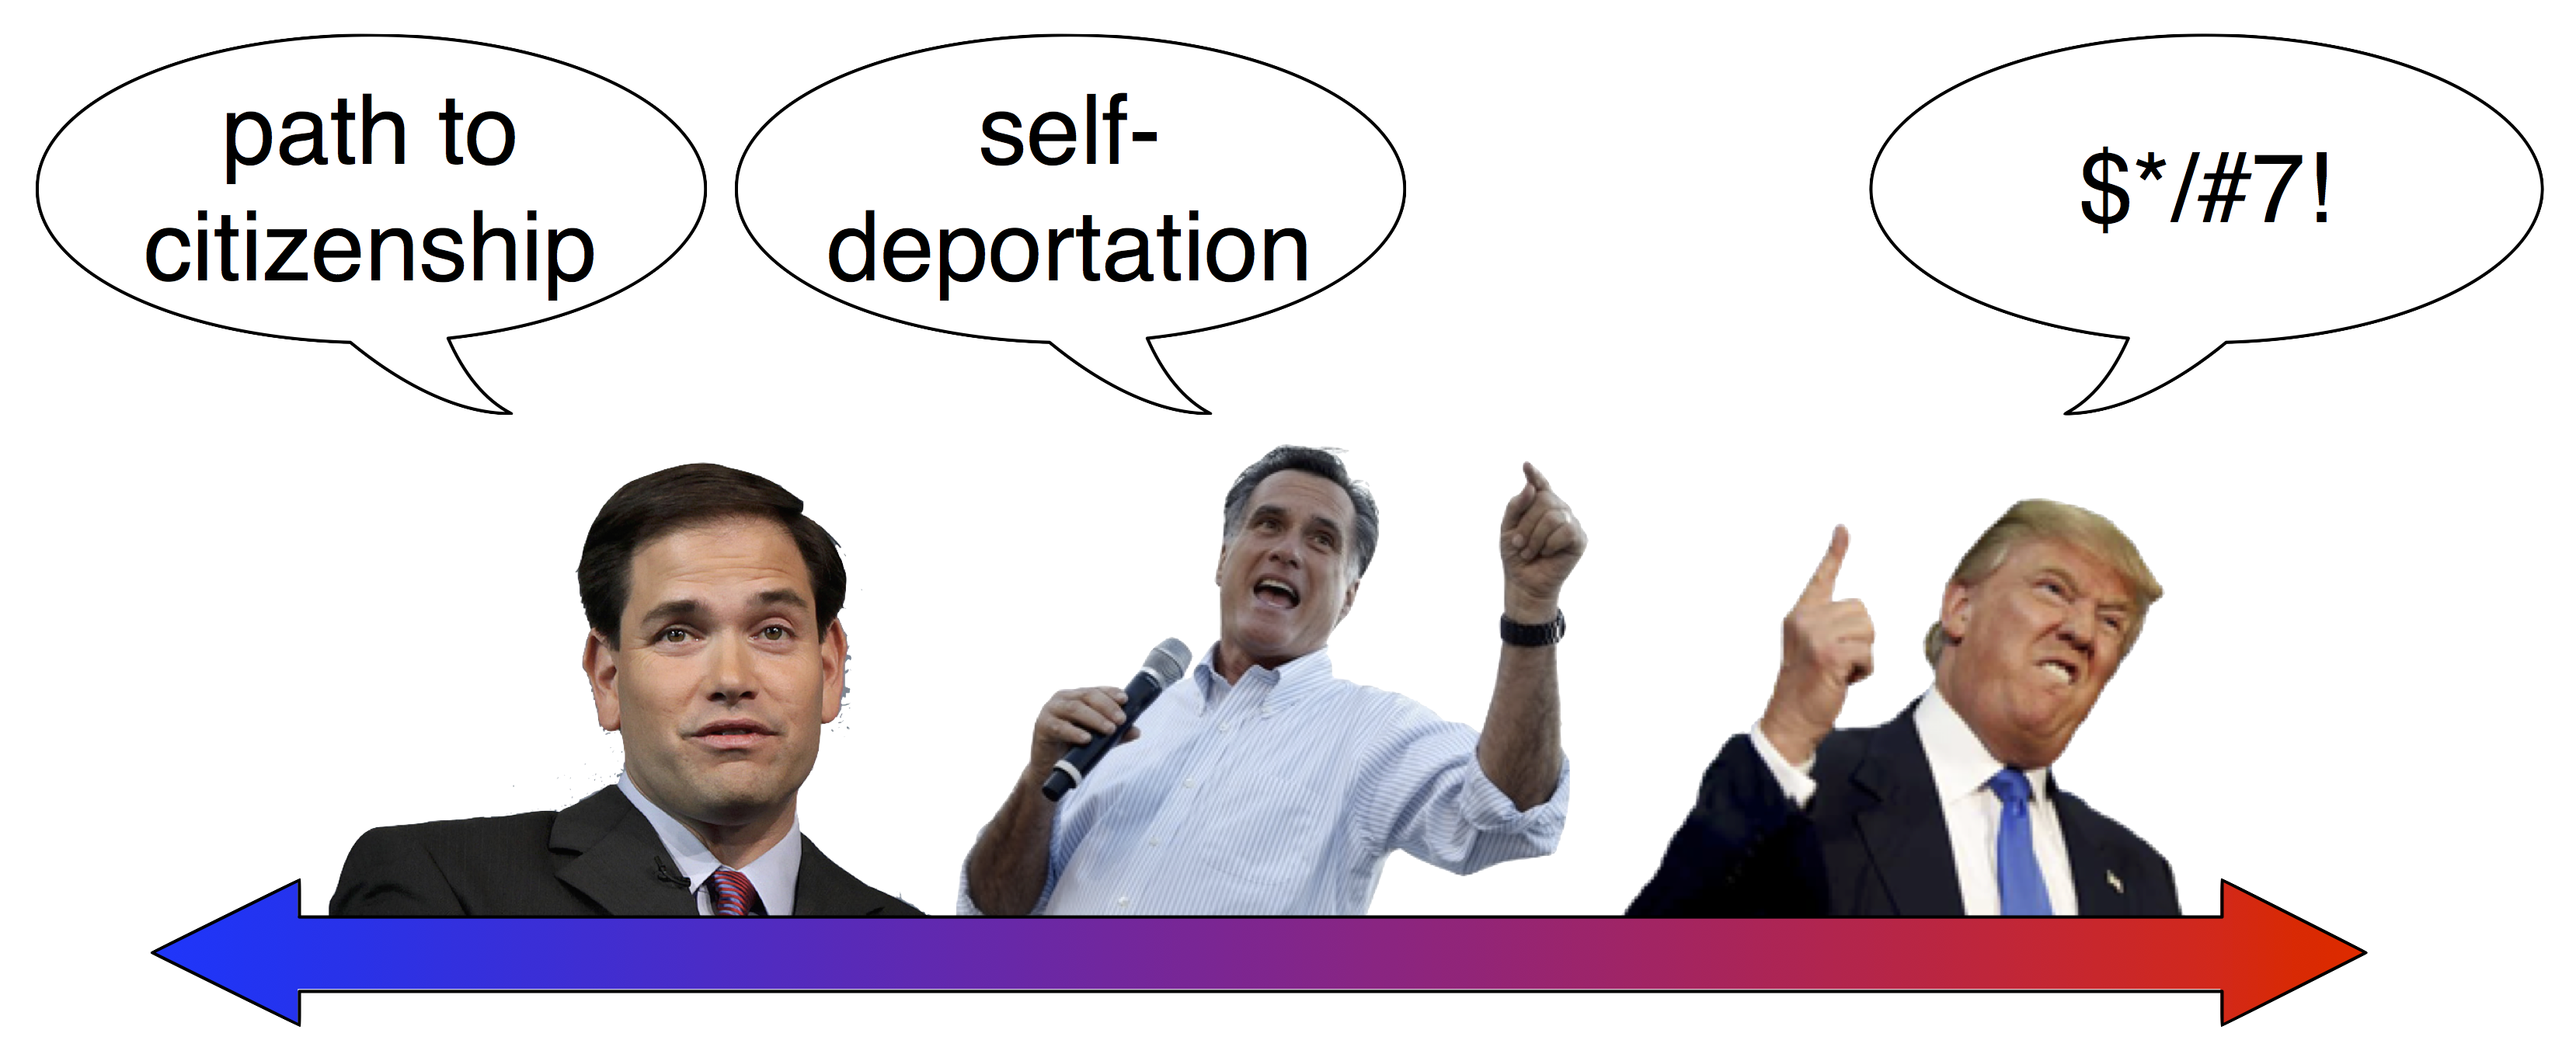
\includegraphics[width=0.9\linewidth]{teaparty/figures/framing} \\
     \cite{nguyen-13b,nguyen-15}
   \end{block}


    \begin{block}{Interactive Machine Learning}
     \centering
        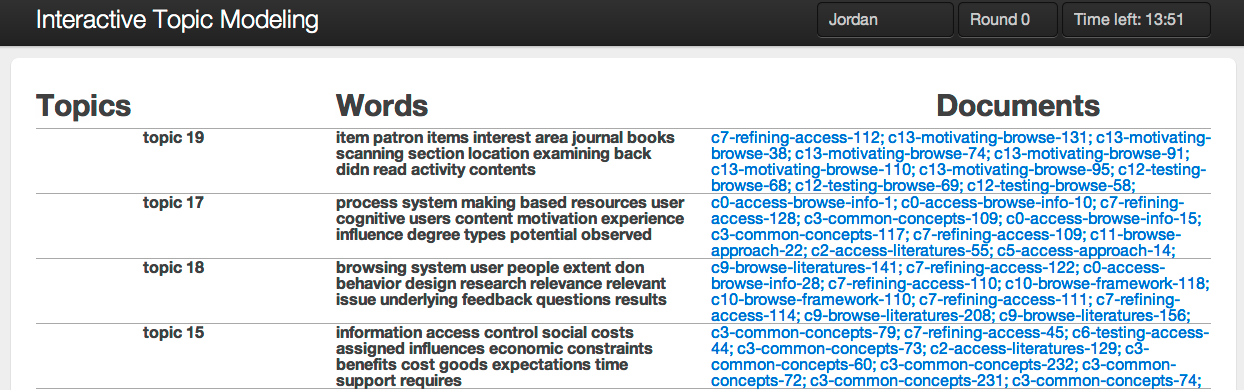
\includegraphics[width=0.4\linewidth]{interactive_topic_models/new_interface} \\
       \cite{boyd-graber-06b,ma-09,nikolova-09}
    \end{block}


  \column{.5\linewidth}


    \begin{block}{Multilingual Topic Models}
      \begin{center}
        \begin{large}
          $p_{\mbox{topic}}(e | f)$ \\
         \end{large}
      \cite{eidelman-12,hu-14}
       \end{center}
    \vspace{-.3cm}
    \end{block}


    \begin{block}{Sentiment / Internal State}
    \centering
        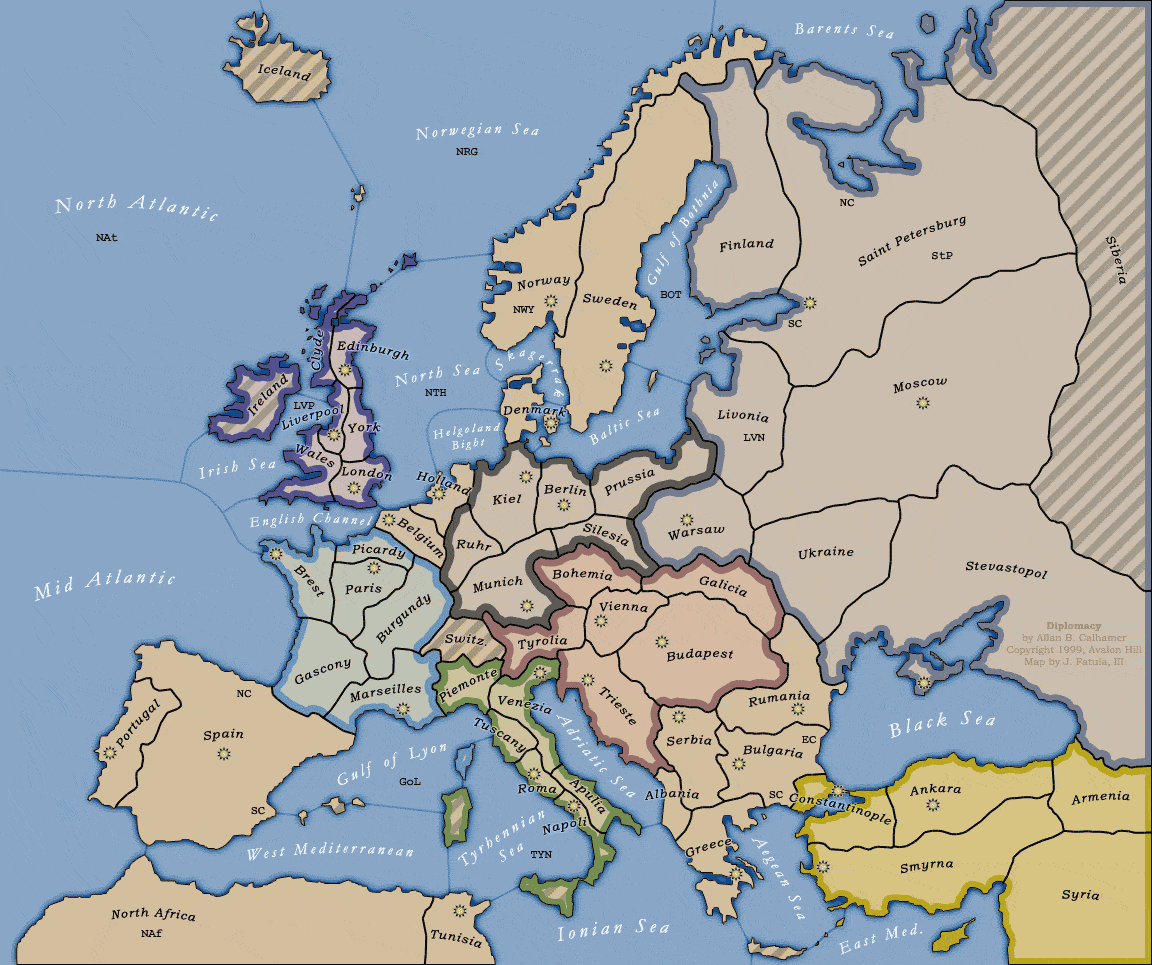
\includegraphics[width=0.4\linewidth]{general_figures/diplomacy} \\
        \cite{niculae-15,sayeed-12,boyd-graber-10}
    \end{block}




\end{columns}

}



\frame{

	\frametitle{Thanks}

        \begin{block}{Collaborators}
          \textsc{naqt}, Hal Daum\'e III (UMD), Anupam Guha (Maryland), Manjhunath Ravi (Colorado), Danny Bouman (UMD UG),
          Stephanie Hwa (UMD UG)
        \end{block}

	\begin{columns}
	
	\column{.5\linewidth}
        \begin{block}{Funders}
        \begin{center}
          
\includegraphics[width=0.4\linewidth]{general_figures/nsf}
       \end{center}
        \end{block}
        
	\column{.5\linewidth}        
        \begin{block}{Supporters}
        	\gfxq{naqt}{.4}
        \end{block}

        \end{columns}
}




\begin{frame}{References}
\bibliographystyle{style/acl}
\tiny
\bibliography{bib/journal-full,bib/jbg}
\end{frame}




	

\begin{frame}
	\frametitle{Learning which Features are Useful}

	\begin{itemize}
		\item Use how humans these data as a prior for supervised maxent model~\cite{daume-04}
		\item Prior for label $a$ and feature $f$ is a function of the number of buzzes $b$ and tf-idf~\cite{salton-68}
\begin{equation}
  \left[ \vphantom{\frac{a}{b}}\alpha \alert<4>{\ind{ b(a,f) > 0}} + \beta \alert<3>{ b(a,f)} + \gamma
  \right] \alert<2>{\mbox{tf-idf}(a,f)} .
\label{eq:meanweight}
\end{equation}
		\begin{itemize}
			\item $\alpha$, $\beta$, and $\gamma = 0$: na\"ive zero prior
			\item $\alpha$ and $\beta = 0$: linear transformation of the mean
			\item $\alpha$ and $\gamma = 0$: number of buzzes times tf-idf value of the features
		\end{itemize}

	\end{itemize}

\end{frame}

\begin{frame}
	\frametitle{Using buzzes as a prior}

\begin{equation*}
  \left[ \vphantom{\frac{a}{b}}\alpha \ind{ b(a,f) > 0} + \beta b(a,f) + \gamma
  \right] \mbox{tf-idf}(a,f) .
\end{equation*}

\begin{center}
\begin{tabular}{cccccc}
Answers & Weighting & $\alpha$ & $\beta$ & $\gamma$ & Error\footnote{Buzz and tf-idf computed on training data; grid search on dev data; error on test data} \\
\hline
\multirow{5}{*}{100} & zero & - & - & - & 0.22 \\
& tf-idf & - & - & 8.3 & 0.08 \\
&  buzz-binary & 10.7 & - & - & {\bf 0.06} \\
&  buzz-linear & - &  1.1 & - & 0.10 \\
& buzz-tier & - & 1.6 & 0.5 & 0.07 \\
\hline
\end{tabular}
\end{center}
\end{frame}





\begin{frame}
	\begin{center}

\vspace{-.6cm}
\begin{figure}[tb]
\centering

\subfigure[Buzzes over all Questions]{
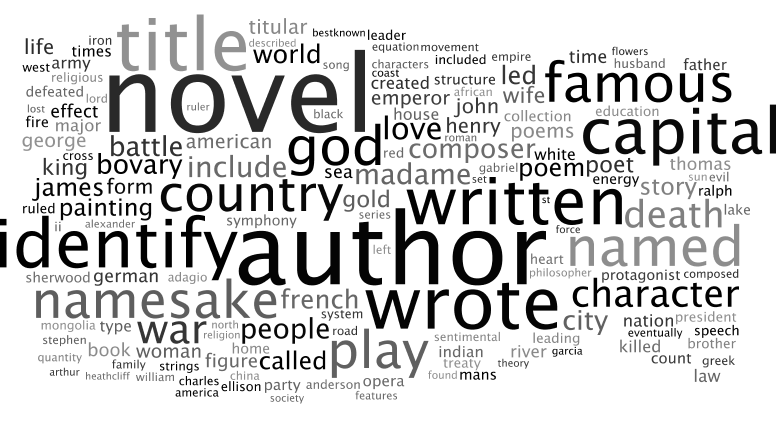
\includegraphics[width=0.6\linewidth]{qb/buzz_cloud}
\label{fig:buzz_cloud}
}

\subfigure[Wuthering Heights Question Text]{
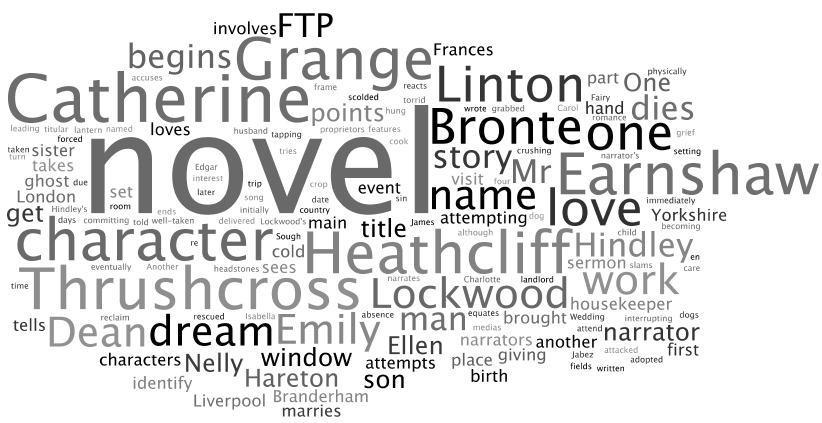
\includegraphics[width=0.45\linewidth]{qb/wuthering_heights_question}
\label{fig:wh_question}
}
\subfigure[Buzzes on Wuthering Heights]{
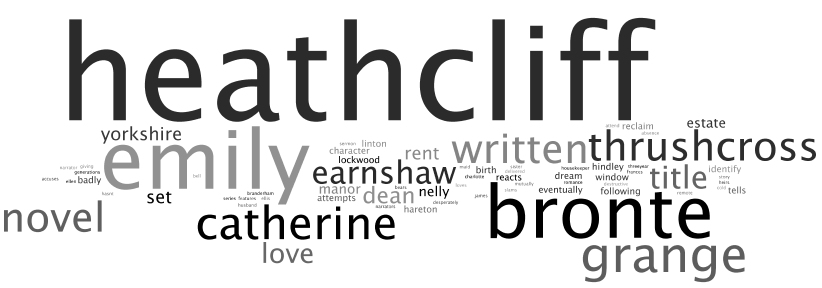
\includegraphics[width=0.45\linewidth]{qb/wuthering_heights_buzz}
\label{fig:wh_buzz}
}
\end{figure}


	\end{center}

\end{frame}



\begin{frame}
	\frametitle{Accuracy vs. Speed}

	\begin{center}
	  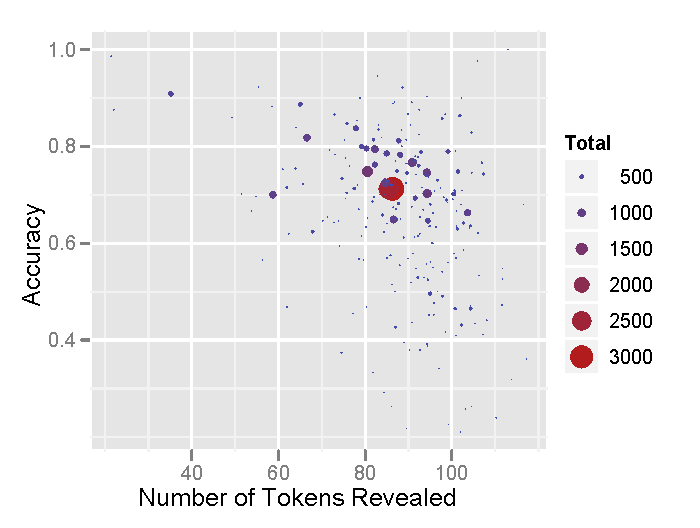
\includegraphics[width=0.8\linewidth]{qb/accuracy_vs_speed}
	  \end{center}

\end{frame}

\begin{frame}{How we could translate a sentence}

\only<1>{\gfxs{example_3}{.9}}
\only<2>{\gfxs{example_4}{.9}}
\only<3>{\gfxs{example_5}{.9}}
\only<4>{\gfxs{example_6}{.9}}
\only<5>{\gfxs{example_7}{.9}}
\only<6>{\gfxs{example_8}{.9}}
\only<7>{\gfxs{example_9}{.9}}
\only<8>{\gfxs{example_10}{.9}}
\only<9>{\gfxs{example_11}{.9}}
\only<10>{\gfxs{example_12}{.9}}
\only<11>{\gfxs{example_13}{.9}}
\only<12>{\gfxs{example_14}{.9}}
\only<13>{\gfxs{example_15}{.9}}
\only<14>{\gfxs{example_16}{.9}}
\only<15>{\gfxs{example_17}{.9}}
\only<16>{\gfxs{example_18}{.9}}
\only<17>{\gfxs{example_19}{.9}}
\end{frame}




\end{document}
